

\chapter[Quant UnivEDA Interp]{Univariate EDA - Quantitative II (Interpretation)} \label{chap:UnivEDAQuant2}
\begin{ChapObj}{\boxwidth}
  \textbf{Objectives:}
  \begin{Enumerate}
    \item Use graphs to describe the shape of a distribution,
    \item Use graphs to describe outliers in a distribution,
    \item Identify which summary statistics are appropriate in a given situation, and
    \item Construct an appropriate overall summary.
  \end{Enumerate}
\end{ChapObj}

\minitoc
\newpage

\lettrine{M}{ethods for constructing numerical and graphical summaries} of a single quantitative variable were discussed in \modref{chap:UnivEDAQuant1}. Those summaries are interpreted here to provide an overall description of the distribution of the quantitative variable

\section{Items to Describe}
A univariate EDA for a quantitative variable is concerned with describing the distribution of the values for that variable; i.e., describing what values occurred and how often those values occurred.\index{EDA!Univariate!Quantitative}  Specifically, the distribution is described by four specific attributes:

\vspace{-12pt}
\begin{Enumerate}
  \item \textbf{shape} of the distribution,
  \item presence of \textbf{outliers},
  \item \textbf{center} of the distribution, and
  \item \textbf{dispersion} or spread of the distribution.
\end{Enumerate}
\vspace{-8pt}

Graphs are used to identify shape and the presence of outliers and to get a general feel for center and dispersion. However, numerical summaries are used to specifically describe center and dispersion of the data.

\vspace{-6pt}
\warn{Shape, center, dispersion, and outliers are described for each quantitative variable.}

\vspace{-12pt}
\warn{Shape and outliers are described from graphs; center and dispersion are describe with numerical summaries.}

The same three data sets used in \modref{chap:UnivEDAQuant1} are used here.

\vspace{-12pt}
\begin{Itemize}
  \item Measurements of water consumption in one hour by mice \tabrefp{tab:MouseData}.
  \item Richter scale recordings for 15 major earthquakes \tabrefp{tab:EQData}.
  \item The number of days of ice cover at ice gauge station 9004 in Lake Superior.
\end{Itemize}

\section{Interpreting Shape}\index{Histogram!Interpretation}
A histogram has two tails -- a left-tail for smaller or more negative values and a right-tail for larger or more positive values. The relative appearance of these two tails is used to identify three different shapes of distributions -- symmetric, left-skewed, and right-skewed.\index{Shape}\index{Symmetric}\index{Skewed}  If the left- and right-tail of a histogram are equal in shape (length and height), then the distribution is said to be \textbf{symmetric}. Perfectly symmetric distributions rarely occur in ``real-life.''  Therefore, if the left- and right-tail are approximately equal in shape, then the distribution is \textbf{approximately symmetric}. If the left-tail of the histogram is stretched out or, alternatively, the left-tail is longer and flatter than the right-tail, then the distribution is negatively- or \textbf{left-skewed}. If the right-tail of the histogram is stretched out or, alternatively, the right-tail is longer and flatter than the left-tail, then the distribution is positively- or \textbf{right-skewed}. The type of skew is defined by the longer tail; a longer right-tail means the distribution is right-skewed and a longer left-tail means it is left-skewed. Examples of each shape are shown in \figref{fig:ShapeExamples}.

\begin{knitrout}
\definecolor{shadecolor}{rgb}{0.969, 0.969, 0.969}\color{fgcolor}\begin{figure}
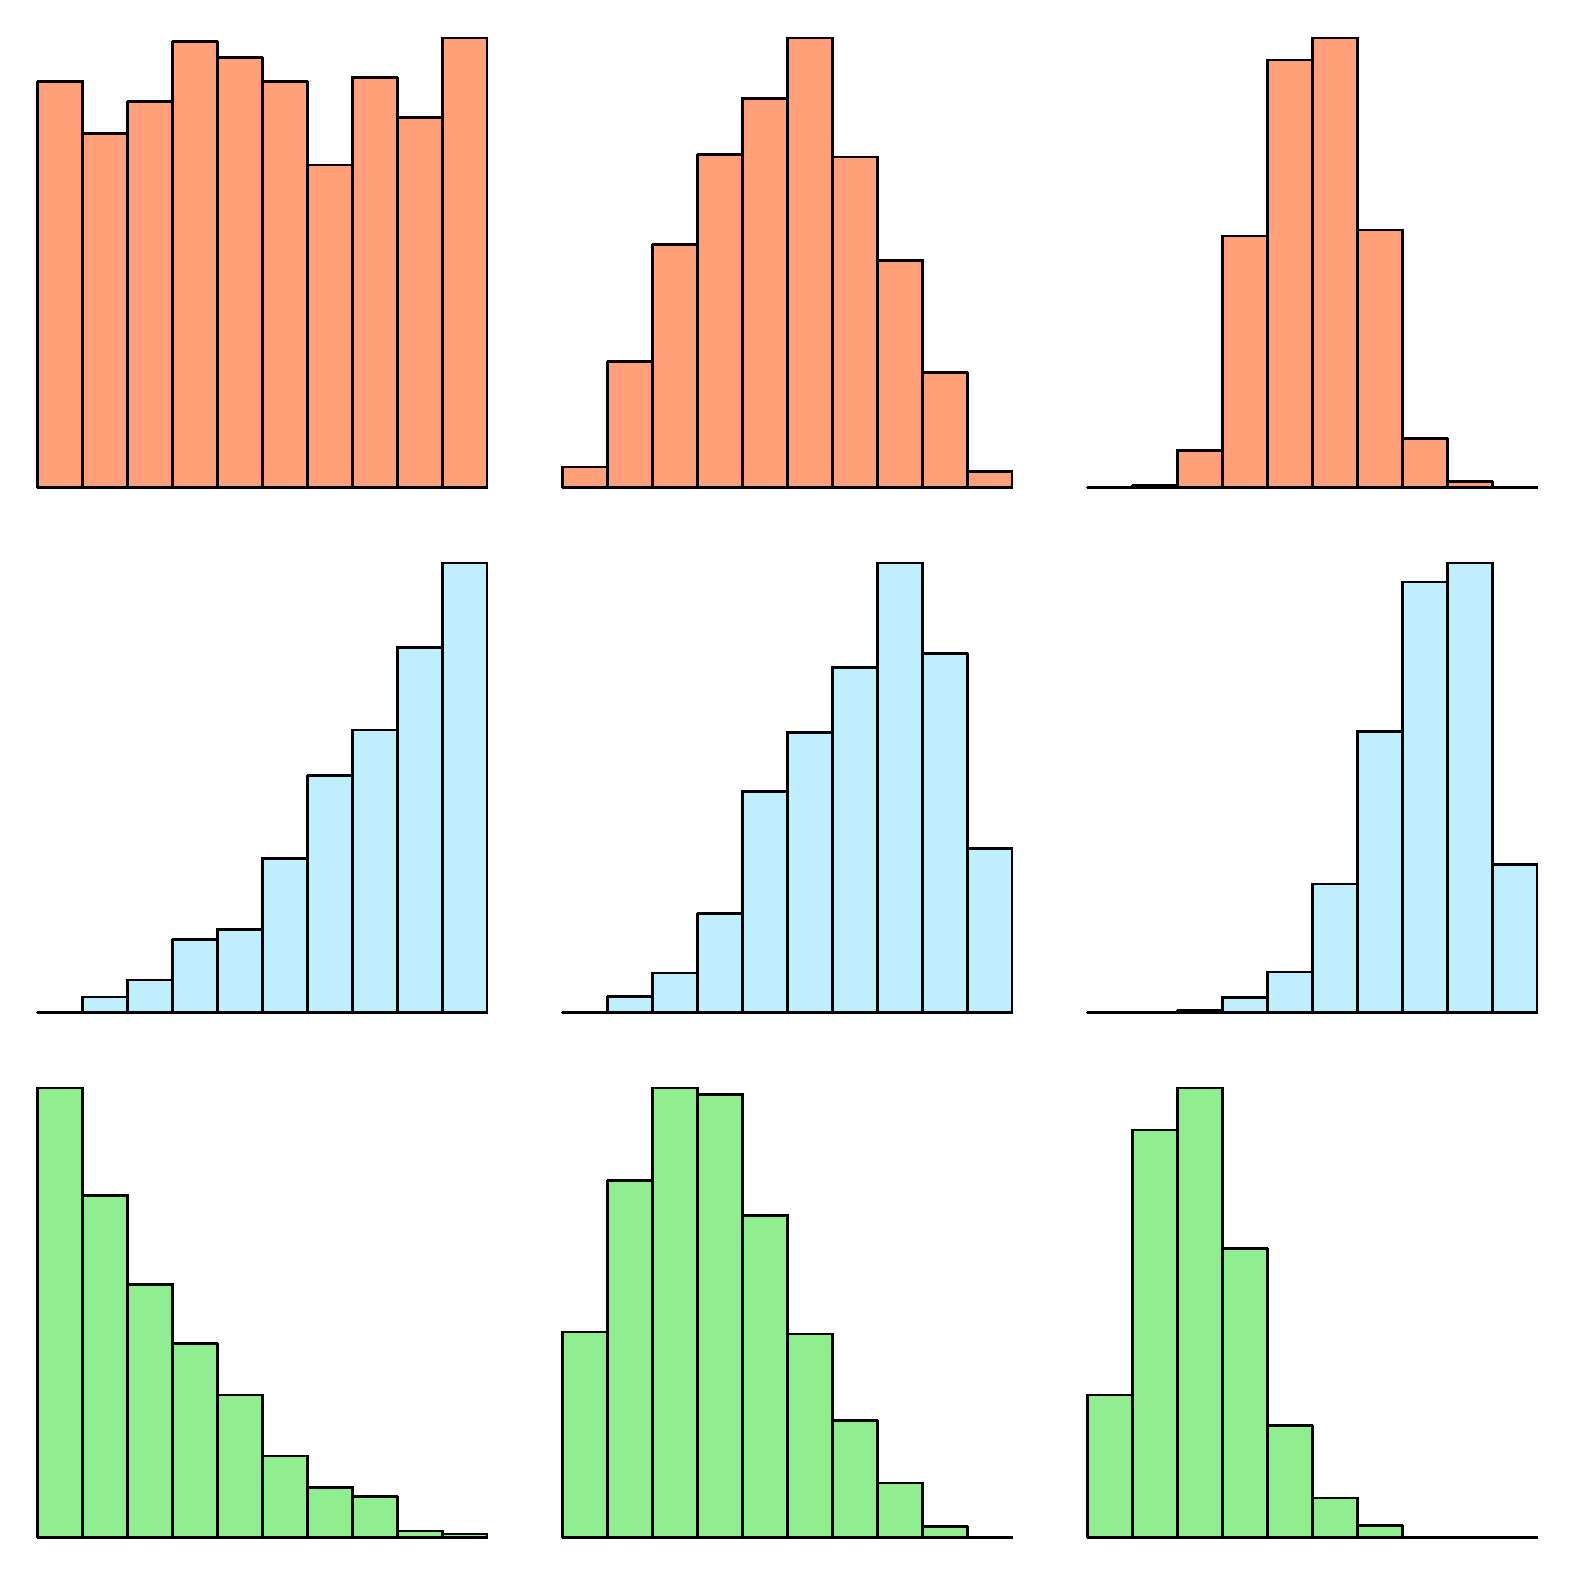
\includegraphics[width=.7\linewidth]{figure/ShapeExamples-1} \caption[Examples of approximately symmetric (top, red), left-skewed (middle, blue), and right-skewed (bottom, green) histograms]{Examples of approximately symmetric (top, red), left-skewed (middle, blue), and right-skewed (bottom, green) histograms. Note that the axes labels were removed to focus attention on the shape of the histograms. Each histogram was constructed from n=1000 individuals and the x-axis range is from 0 to 1.}\label{fig:ShapeExamples}
\end{figure}


\end{knitrout}

\defn{Symmetric}{The left- and right-tail of a distribution are nearly the same in length and height.}

\vspace{-12pt}
\defn{Left-skewed}{The left-tail of a distribution is longer or more drawn out than the right-tail.}

\vspace{-12pt}
\defn{Right-skewed}{The right-tail of a distribution is longer or more drawn out than the left-tail.}

\vspace{-12pt}
\warn{The longer tail defines the type of skew.}

In practice, these labels form a continuum. For example, a perfectly symmetric distribution is rare. However, in the many cases of an asymmetric distribution, it is a fine line between calling the shape approximately symmetric or one of the skewed distributions.

\vspace{-12pt}
\warn{Symmetric, left-skewed, and right-skewed descriptors are guides; many ``real'' distributions will not fall neatly into these categories.}

The relative length from the median to Q1 and the median to Q3 (i.e., the position of the median line in the box) indicates the shape of the distribution.\index{Boxplot!Interpretation}  If the distribution is left-skewed (i.e., lesser-valued individuals are ``spread out''; \figref{fig:BoxplotShape}-Right), then median-Q1 will be greater than Q3-median. In contrast, if the distribution is right-skewed (i.e., larger-valued individuals are spread out; \figref{fig:BoxplotShape}-Middle), then Q3-median will be greater than median-Q1. Thus, if the distribution is right-skewed then the median will be closer to Q1 than to Q3, if the distribution is left-skewed then the median will be closer to Q3 than to Q1, and if the distribution is approximately symmetric (\figref{fig:BoxplotShape}-Left) then the median will be in the middle of the box.

\begin{knitrout}
\definecolor{shadecolor}{rgb}{0.969, 0.969, 0.969}\color{fgcolor}\begin{figure}
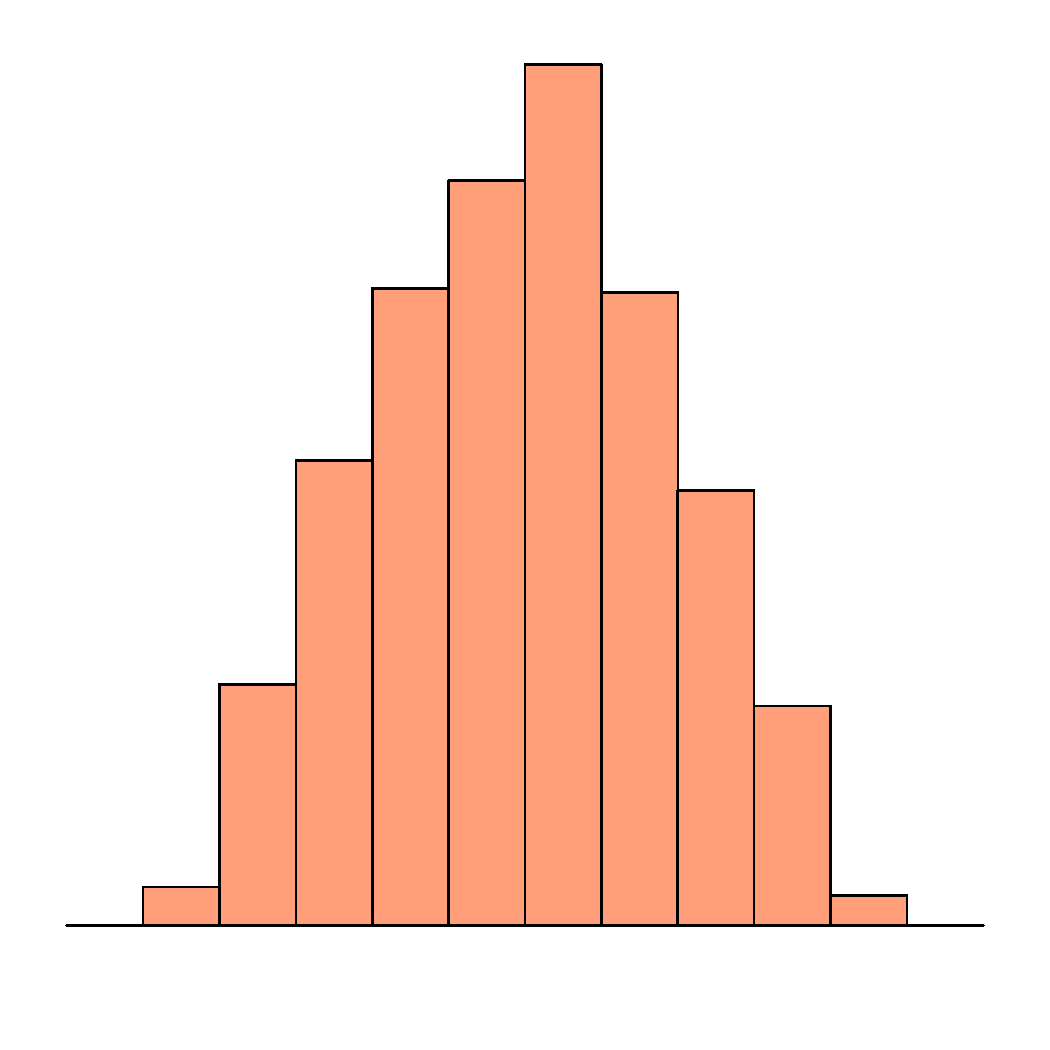
\includegraphics[width=.3\linewidth]{figure/BoxplotShape-1} \caption[Histograms and boxplots for several different shapes of distributions]{Histograms and boxplots for several different shapes of distributions.}\label{fig:BoxplotShape1}
\end{figure}

\begin{figure}
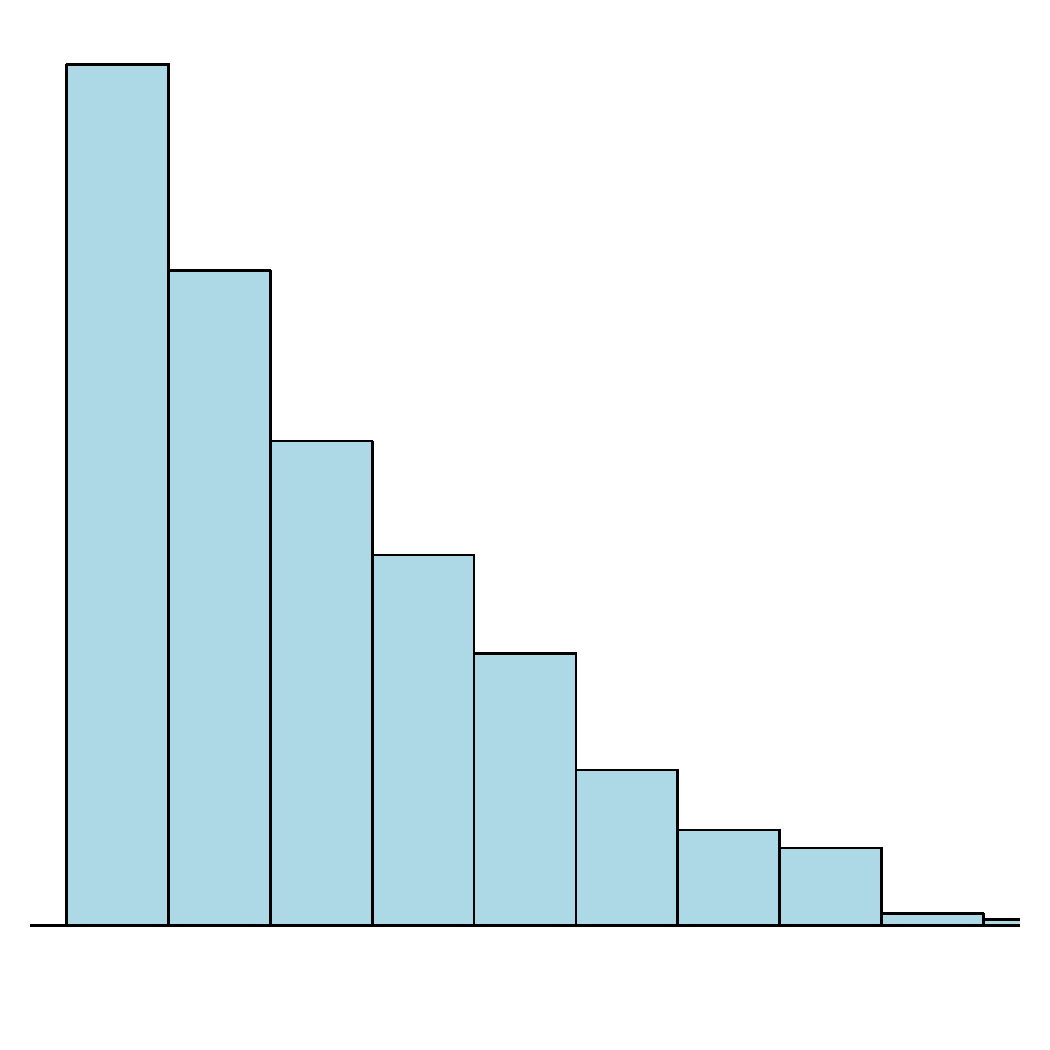
\includegraphics[width=.3\linewidth]{figure/BoxplotShape-2} \caption[Histograms and boxplots for several different shapes of distributions]{Histograms and boxplots for several different shapes of distributions.}\label{fig:BoxplotShape2}
\end{figure}

\begin{figure}
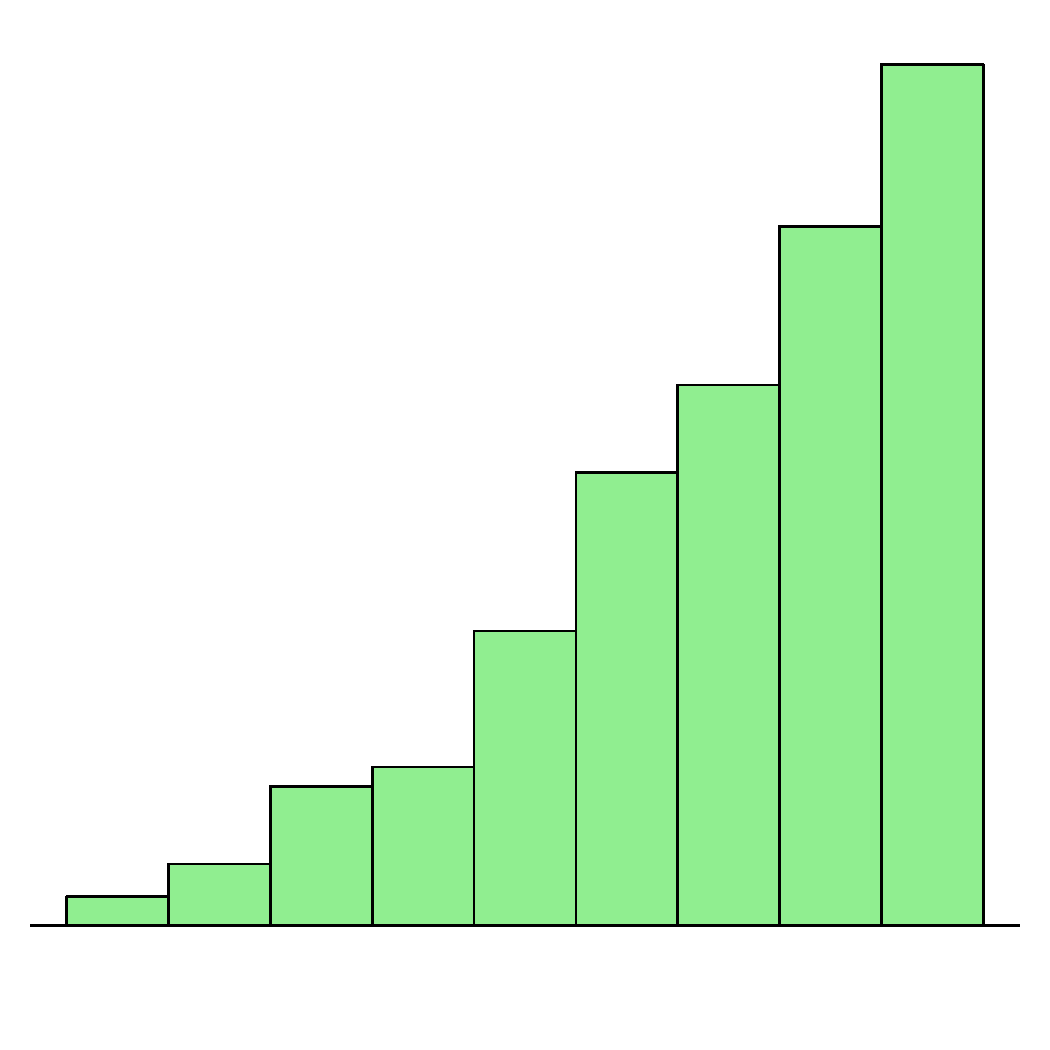
\includegraphics[width=.3\linewidth]{figure/BoxplotShape-3} \caption[Histograms and boxplots for several different shapes of distributions]{Histograms and boxplots for several different shapes of distributions.}\label{fig:BoxplotShape3}
\end{figure}

\begin{figure}
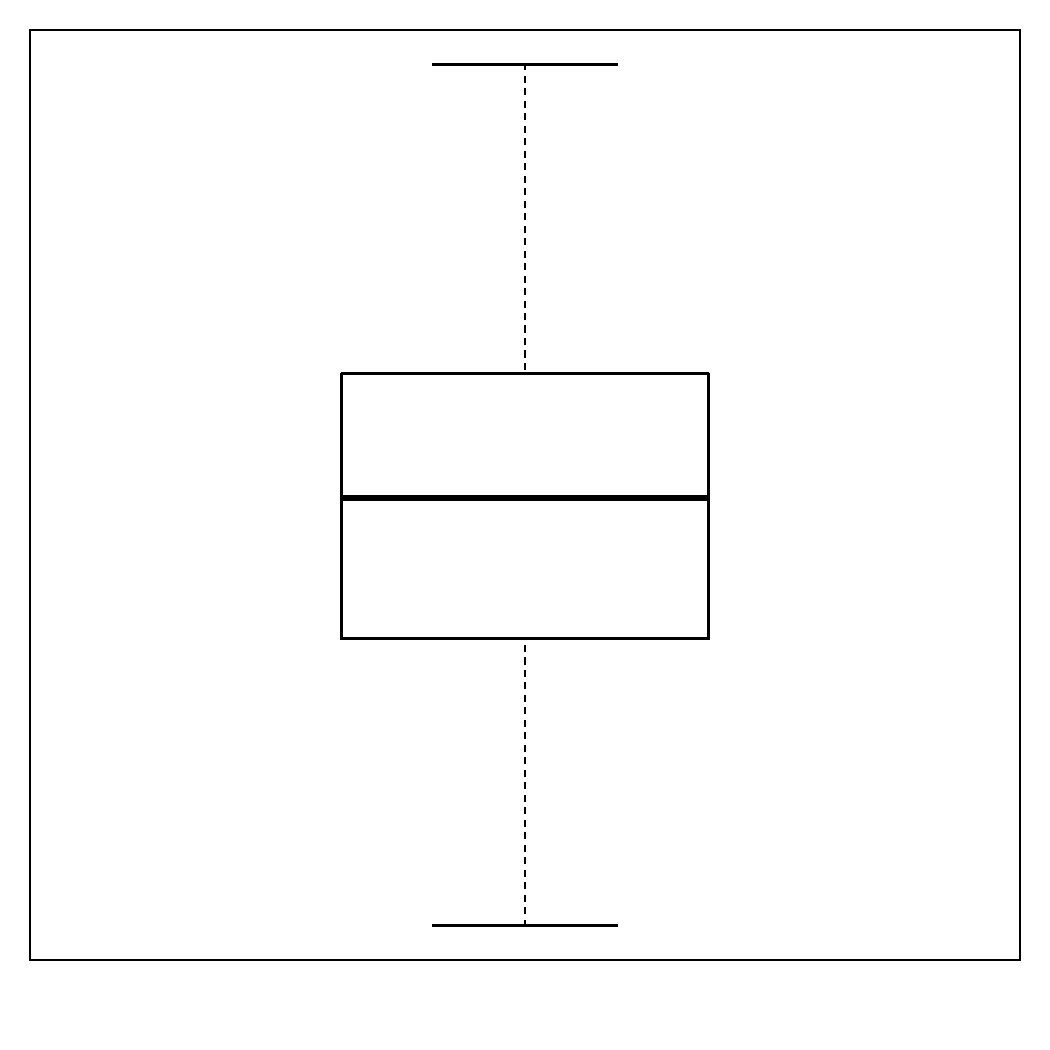
\includegraphics[width=.3\linewidth]{figure/BoxplotShape-4} \caption[Histograms and boxplots for several different shapes of distributions]{Histograms and boxplots for several different shapes of distributions.}\label{fig:BoxplotShape4}
\end{figure}

\begin{figure}
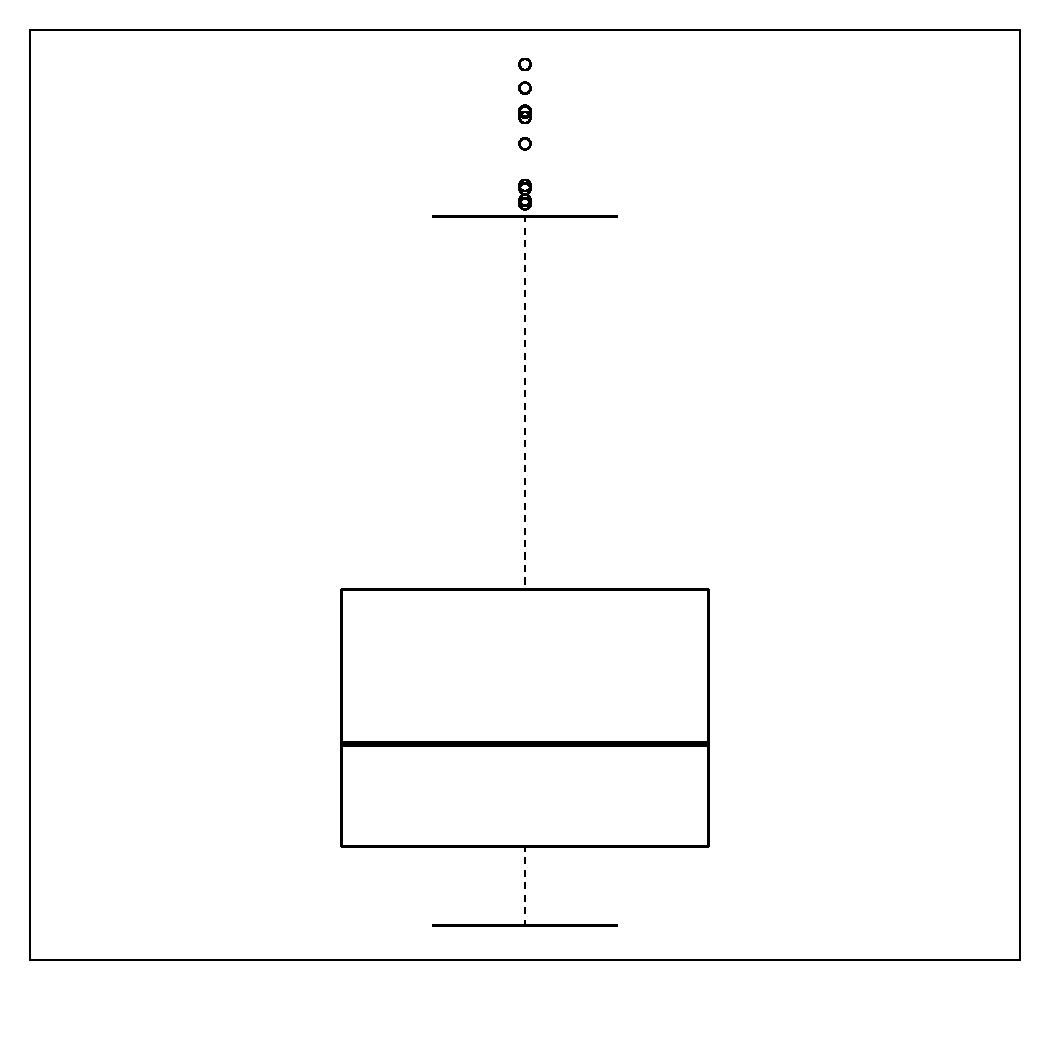
\includegraphics[width=.3\linewidth]{figure/BoxplotShape-5} \caption[Histograms and boxplots for several different shapes of distributions]{Histograms and boxplots for several different shapes of distributions.}\label{fig:BoxplotShape5}
\end{figure}

\begin{figure}
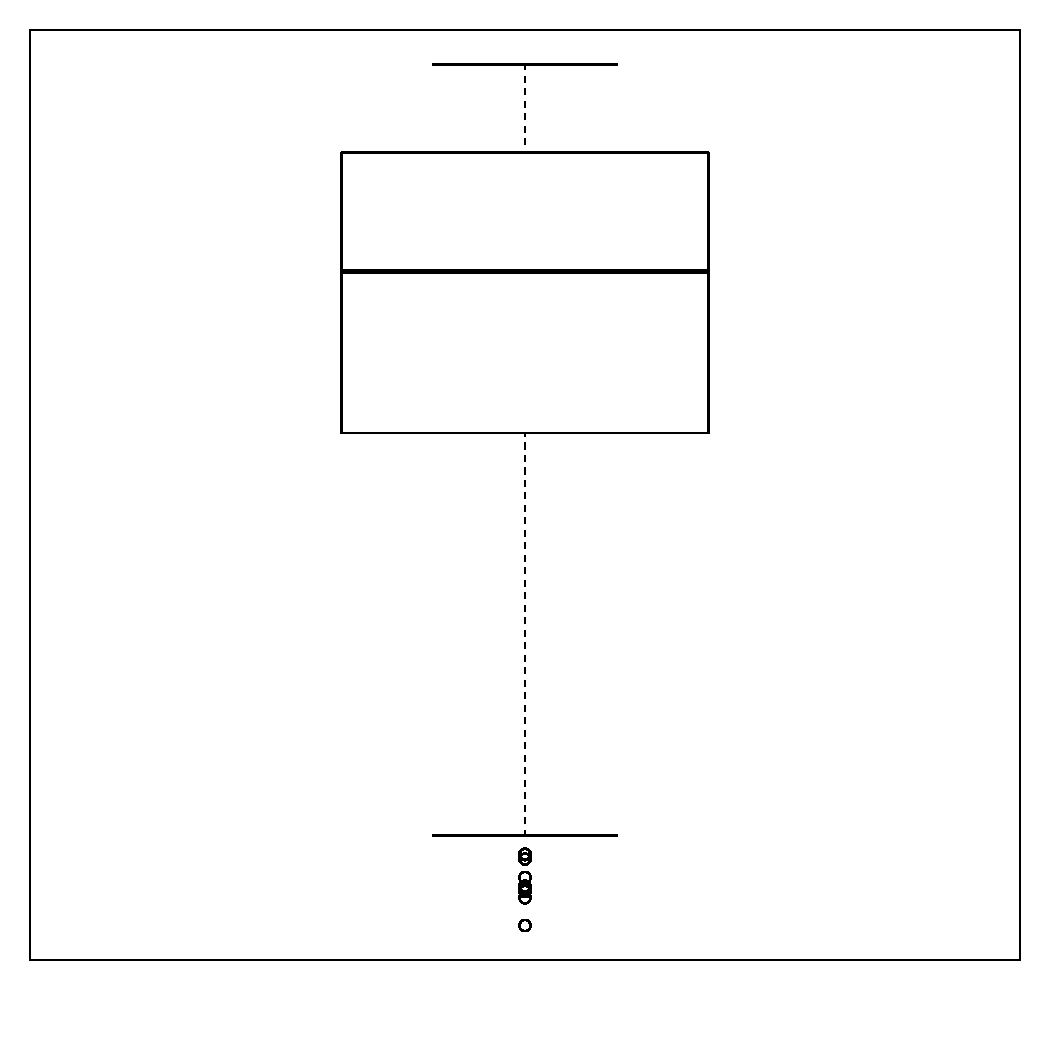
\includegraphics[width=.3\linewidth]{figure/BoxplotShape-6} \caption[Histograms and boxplots for several different shapes of distributions]{Histograms and boxplots for several different shapes of distributions.}\label{fig:BoxplotShape6}
\end{figure}


\end{knitrout}

\warn{If a distribution is right-skewed, then the median will be closer to Q1 than to Q3. If the distribution is left-skewed, then the median will be closer to Q3 than to Q1.}

\vspace{-12pt}
\warn{Even though shape can be described from a boxplot, it is always easier to describe shape from a histogram.}

\begin{exsection}
  \item \label{revex:quEDABrule5N} What is the five-number summary for the maximum gauge heights of the Bois Brule River in Brule, WI from Exercise \ref{revex:quEDABrule}. \ansref{ans:quEDABrule5N}
  \item \label{revex:quEDAWI5N} \rhw{} Construct a boxplot for the population density of Wisconsin counties from Exercise \ref{revex:quEDAWIc}. \ansref{ans:quEDAWI5N}
  \item \label{revex:quEDABoxLeft} What is the shape of the left boxplot below? \ansref{ans:quEDABoxLeft}

\begin{center}
  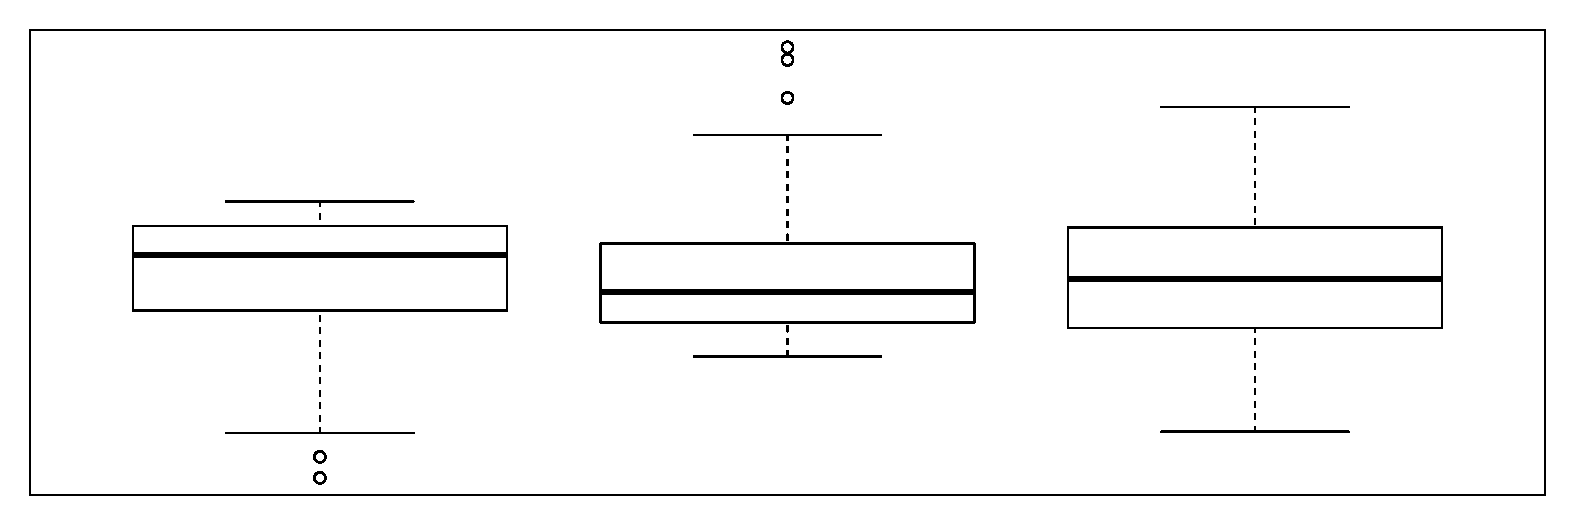
\includegraphics[width=4in]{Figs/BoxplotQuest-1}
\end{center}

  \item \label{revex:quEDABoxRight} What is the shape of the middle boxplot above? \ansref{ans:quEDABoxRight}
  \item \label{revex:quEDABoxSym} What is the shape of the right boxplot above? \ansref{ans:quEDABoxSym}
  \item \label{revex:quEDALSkewCtr} If the distribution is skewed left, which measure should you generally use to measure center? \ansref{ans:quEDALSkewCtr}
  \item \label{revex:quEDARSkewCtr} Which measure of center should you generally use for a right-skewed distribution? \ansref{ans:quEDARSkewCtr}
  \item \label{revex:quEDASymCtr} Which measure of center should you generally use for a symmetric distribution? \ansref{ans:quEDASymCtr}
  \item \label{revex:quEDASymDisp} Which measure of dispersion should you generally use for a symmetric distribution? \ansref{ans:quEDASymDisp}
  \item \label{revex:quEDALSkewDisp} Which measure of dispersion should you generally use for a left-skewed distribution? \ansref{ans:quEDALSkewDisp}
  \item \label{revex:quEDARSkewDisp} Which measure of dispersion should you generally use for a right-skewed distribution? \ansref{ans:quEDARSkewDisp}
  \item \label{revex:quEDAQShape1} Is Q3-Q2 less than, approximately equal to, or greater than Q2-Q1 if the data are left-skewed? \ansref{ans:quEDAQShape1}
  \item \label{revex:quEDAQShape2} What is the shape of the distribution if Q3-Q2 is greater than Q2-Q1? \ansref{ans:quEDAQShape2}
\end{exsection}


\section{Interpreting Outliers}\index{Outlier}\index{Histogram!Interpretation}
An outlier is an individual whose value is widely separated from the main cluster of values in the sample. On histograms, outliers appear as bars that are separated from the main cluster of bars by ``white space'' or areas with no bars \figrefp{fig:OutlierExHist}. In general, outliers must be on the margins of the histogram, should be separated by one or two missing bars, and should only be one or two individuals.

\begin{knitrout}
\definecolor{shadecolor}{rgb}{0.969, 0.969, 0.969}\color{fgcolor}\begin{figure}
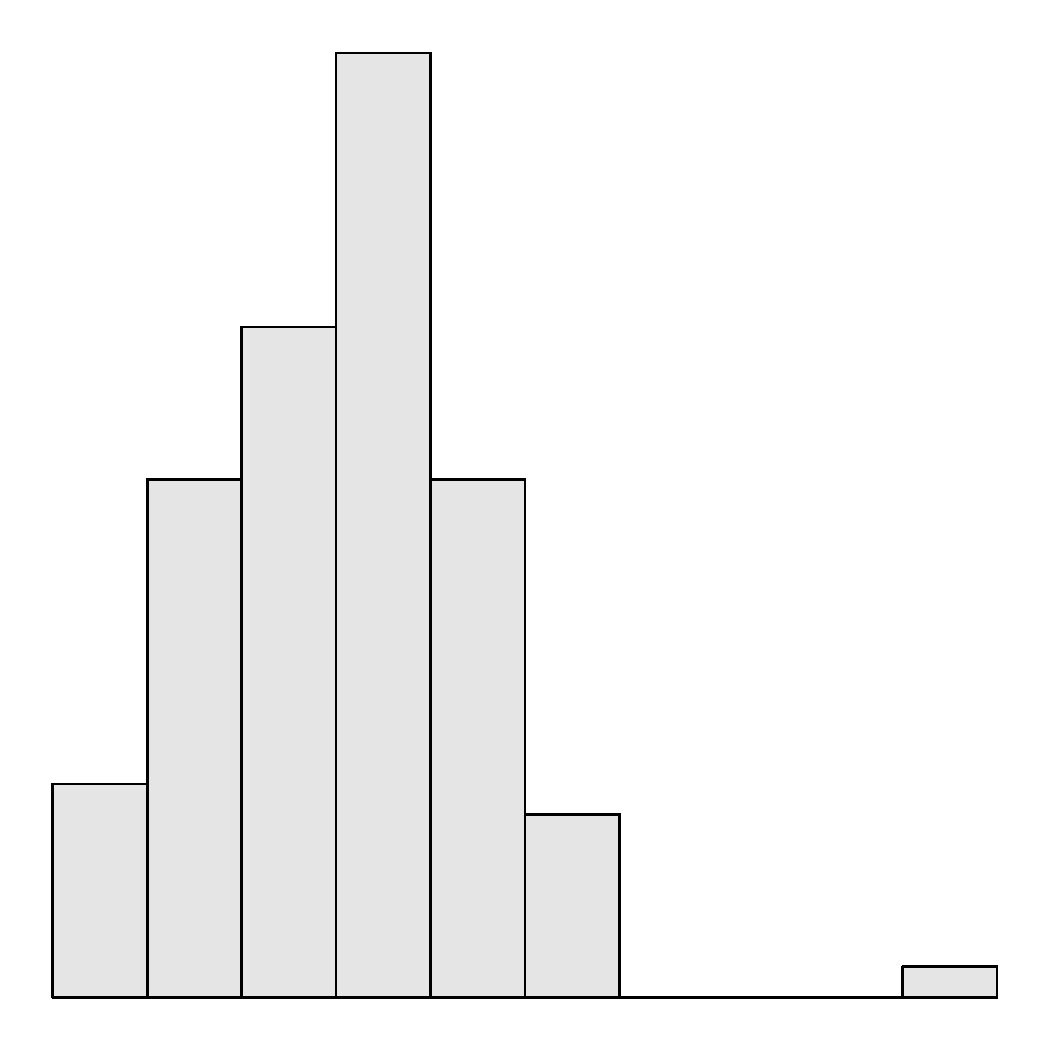
\includegraphics[width=\maxwidth]{figure/OutlierExHist-1} \caption[Example histogram with an outlier to the right]{Example histogram with an outlier to the right.}\label{fig:OutlierExHist}
\end{figure}


\end{knitrout}

\defn{Outlier}{An individual whose value is widely separated from the main cluster of values in the sample.}

An outlier may occur as a result of human error in the sampling process. If this is the case, then the value should be corrected or removed. Other times an outlier may be an individual that was not part of the population of interest -- e.g., an adult animal that was sampled when only immature animals were being considered. In this case, the individual's value should be removed from the sample. Still other times, an outlier is part of the population and should generally not be removed from the sample. In fact you may wish to highlight an outlier as an interesting observation! Regardless, it is important that you construct a histogram to determine if outliers are present or not.

Don't let outliers completely influence how you define the shape of a distribution. For example, if the main cluster of values is approximately symmetric and there is one outlier to the right of the main cluster (as illustrated in \figref{fig:OutlierExHist}), \textbf{DON'T} call the distribution right-skewed. You should describe this distribution as approximately symmetric with an outlier to the right.

\warn{Not all outliers warrant removal from your sample.}

\vspace{-12pt}
\warn{Don't let outliers completely influence how you define the shape of a distribution.}

\vspace{24pt}
\begin{exsection}
  \item \label{revex:quEDALSkew} What is a distribution with a long left-tail called? \ansref{ans:quEDALSkew}
  \item \label{revex:quEDARSkew} What is a distribution with a long right-tail called? \ansref{ans:quEDARSkew}
  \item \label{revex:quEDALSkewg} What is the shape of the distribution on the left below? \ansref{ans:quEDALSkewg}


\begin{center}
  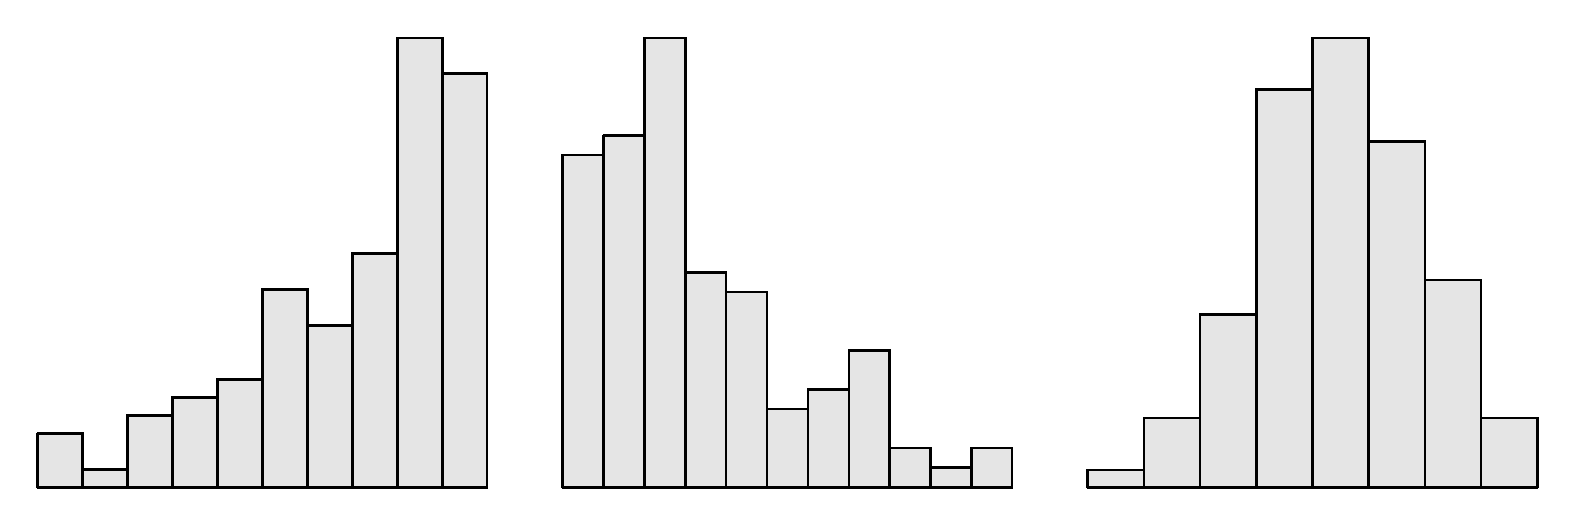
\includegraphics[width=5in]{Figs/HistQuest-1}
\end{center}
  \item \label{revex:quEDASymg} What is the shape of the distribution in the center above? \ansref{ans:quEDASymg}
  \item \label{revex:quEDARSkewg} What is the shape of the distribution on the right above? \ansref{ans:quEDARSkewg}
  \item \label{revex:quEDAlead} Comment on the shape and presence of outliers in \figref{fig:KreherParkPbhist}. \ansref{ans:quEDAlead}
\end{exsection}


\section{Comparing the Median and Mean} \label{sect:MeanMedian}
The mean and median measure center in different ways.\index{Median!Compared to mean}\index{Mean!Compared to median}\index{Mean!How measures center}\index{Median!How measures center}  The median is concerned with the \textbf{position} of the value rather than the value itself (recall how it is calculated). The mean, on the other hand, is the value such that the sum of the distances from it to all points smaller than it is the same as the sum of the distances from it to all points greater than it. The mean is very much concerned about the \textbf{values} for each individual, as the values are used to find the ``distance'' from the mean.

\warn{The actual values of the data (beyond ordering the data) are not considered when calculating the median; whereas the actual values are very much considered when calculating the mean.}

A plot of the Richter scale data against the corresponding ordered individual number is shown in \figref{fig:MeanMedianComp1}-Left.\footnote{This is a rather non-standard graph but it is useful for comparing how the mean and median measure the center of the data.}  The median (blue line) is found by locating the middle position on the individual number axis and then finding the corresponding Richter scale value (move right until the point is intercepted and then move down to the x-axis). The vertical blue line represents the median, and it can be seen that it has the same \textbf{number} of individuals (i.e., points) below it as above it. In contrast, the mean finds the Richter scale value that has the same total distance to values below it as total distance to values above it. In other words, the mean is the vertical red line so that the total \textbf{length} of the horizontal dashed red lines is the same to the left as it is to the right. Thus, the median balances the number of individuals above and below the median, whereas the mean balances the difference in values above and below the mean.

\begin{knitrout}
\definecolor{shadecolor}{rgb}{0.969, 0.969, 0.969}\color{fgcolor}\begin{kframe}


{\ttfamily\noindent\bfseries\color{errorcolor}{\#\# Error in plot(EQ, 1:length(EQ), pch = 16, ylab = "{}Individual Number"{}, : object 'EQ' not found}}

{\ttfamily\noindent\bfseries\color{errorcolor}{\#\# Error in axis(1, c(5.5, 6, 8)): plot.new has not been called yet}}

{\ttfamily\noindent\bfseries\color{errorcolor}{\#\# Error in axis(2, seq(0, 15, 5)): plot.new has not been called yet}}

{\ttfamily\noindent\bfseries\color{errorcolor}{\#\# Error in text.default(5.15, 8.7, "{}MP="{}, col = "{}blue"{}, xpd = TRUE): plot.new has not been called yet}}

{\ttfamily\noindent\bfseries\color{errorcolor}{\#\# Error in text.default(5.15, 7.5, "{}8"{}, col = "{}blue"{}, xpd = TRUE): plot.new has not been called yet}}

{\ttfamily\noindent\bfseries\color{errorcolor}{\#\# Error in lines(c(0, EQ[8]), c(8, 8), lwd = 2, lty = 2, col = "{}blue"{}): object 'EQ' not found}}

{\ttfamily\noindent\bfseries\color{errorcolor}{\#\# Error in lines(c(EQ[8], EQ[8]), c(8, -1), lwd = 2, lty = 2, col = "{}blue"{}): object 'EQ' not found}}

{\ttfamily\noindent\bfseries\color{errorcolor}{\#\# Error in text(EQ[8], -1.3, "{}Median=7.10"{}, xpd = TRUE, col = "{}blue"{}): object 'EQ' not found}}

{\ttfamily\noindent\bfseries\color{errorcolor}{\#\# Error in mean(EQ): object 'EQ' not found}}

{\ttfamily\noindent\bfseries\color{errorcolor}{\#\# Error in int\_abline(a = a, b = b, h = h, v = v, untf = untf, ...): object 'avg' not found}}

{\ttfamily\noindent\bfseries\color{errorcolor}{\#\# Error in text(avg, -2.7, "{}Mean=7.07"{}, xpd = TRUE, col = "{}red"{}): object 'avg' not found}}

{\ttfamily\noindent\bfseries\color{errorcolor}{\#\# Error in eval(expr, envir, enclos): object 'EQ' not found}}

{\ttfamily\noindent\bfseries\color{errorcolor}{\#\# Error in eval(expr, envir, enclos): object 'EQ' not found}}

{\ttfamily\noindent\bfseries\color{errorcolor}{\#\# Error in plot(EQ1, 1:length(EQ1), pch = 19, ylab = "{}Individual Number"{}, : object 'EQ1' not found}}

{\ttfamily\noindent\bfseries\color{errorcolor}{\#\# Error in axis(1, c(12, 14, 16, 18)): plot.new has not been called yet}}

{\ttfamily\noindent\bfseries\color{errorcolor}{\#\# Error in axis(2, seq(0, 15, 5)): plot.new has not been called yet}}

{\ttfamily\noindent\bfseries\color{errorcolor}{\#\# Error in text.default(3.5, 8.7, "{}MP="{}, col = "{}blue"{}, xpd = TRUE): plot.new has not been called yet}}

{\ttfamily\noindent\bfseries\color{errorcolor}{\#\# Error in text.default(3.5, 7.5, "{}8.5"{}, col = "{}blue"{}, xpd = TRUE): plot.new has not been called yet}}

{\ttfamily\noindent\bfseries\color{errorcolor}{\#\# Error in plot.xy(xy.coords(x, y), type = type, ...): plot.new has not been called yet}}

{\ttfamily\noindent\bfseries\color{errorcolor}{\#\# Error in plot.xy(xy.coords(x, y), type = type, ...): plot.new has not been called yet}}

{\ttfamily\noindent\bfseries\color{errorcolor}{\#\# Error in text.default(med, -1.3, "{}Median=7.20"{}, xpd = TRUE, col = "{}blue"{}): plot.new has not been called yet}}

{\ttfamily\noindent\bfseries\color{errorcolor}{\#\# Error in mean(EQ1): object 'EQ1' not found}}

{\ttfamily\noindent\bfseries\color{errorcolor}{\#\# Error in int\_abline(a = a, b = b, h = h, v = v, untf = untf, ...): object 'avg' not found}}

{\ttfamily\noindent\bfseries\color{errorcolor}{\#\# Error in text(avg, -2.7, "{}Mean=7.81"{}, xpd = TRUE, col = "{}red"{}): object 'avg' not found}}

{\ttfamily\noindent\bfseries\color{errorcolor}{\#\# Error in eval(expr, envir, enclos): object 'EQ1' not found}}\end{kframe}
\end{knitrout}

\warn{The mean balances the distance to individuals above and below the mean. The median balances the number of individuals above and below the median.}

\vspace{-12pt}
\warn{The sum of all differences between individual values and the mean (as properly calculated) equals zero.}

The mean and median differ in their sensitivity to outliers (\figref{fig:MeanMedianComp1}-Right).\index{Mean!Sensitivity to outliers}\index{Median!Sensitivity to outliers}  For example, suppose that an incredible earthquake with a Richter Scale value of 19.0 was added to the earthquake data set. With this additional individual, the median increases from 7.1 to 7.2, but the mean increases from 7.1 to 7.8. The outlier affects the value of the mean more than it affects the value of the median because of the way that each statistic measures center. The mean will be pulled towards an outlier because it must ``put'' many values on the ``side'' of the mean away from the outlier so that the sum of the differences to the larger values and the sum of the differences to the smaller values will be equal. Thus, the outlier in this example creates a large difference to the right of the mean so the mean has to ``move'' to the right to make this difference smaller, move more individuals to the left side of the mean, and increase the differences of individuals to the left of the mean to balance this one large individual. The median on the other hand will simply ``put'' one more individual on the side opposite of the outlier because it balances the number of individuals on each side of it. Thus, the median has to move very little to the right to accomplish this balance.

\warn{The mean is more sensitive (i.e., changes more) to outliers than the median; it will be ``pulled'' towards the outlier more than the median.}

The shape of the distribution, even if outliers are not present, also has an effect on the values of the mean and median as depicted in \figref{fig:MeanMedianShape}. If a distribution is perfectly symmetric, then the median and mean (along with the mode) will be identical. If the distribution is approximately symmetric, then the median and mean will be approximately equal. If the distribution is right-skewed, then the mean will be greater than the median. Finally, if the distribution is left-skewed, then the mean will be less than the median.

\begin{knitrout}
\definecolor{shadecolor}{rgb}{0.969, 0.969, 0.969}\color{fgcolor}\begin{figure}
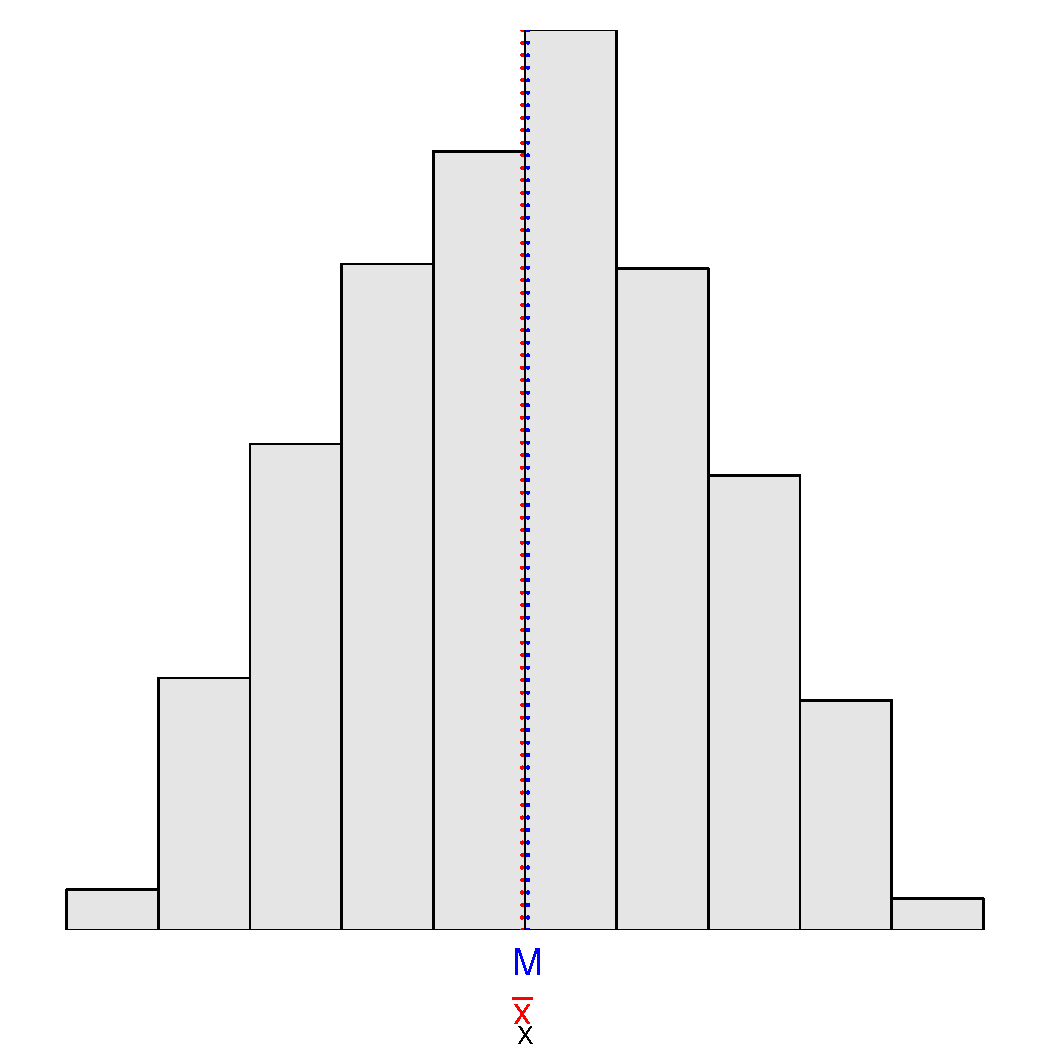
\includegraphics[width=.3\linewidth]{figure/MeanMedianShape-1} \caption[Three differently shaped histograms with vertical lines superimposed at the median (M]{Three differently shaped histograms with vertical lines superimposed at the median (M; blue lines) and the mean ($\bar{x}$; red lines).}\label{fig:MeanMedianShape1}
\end{figure}

\begin{figure}
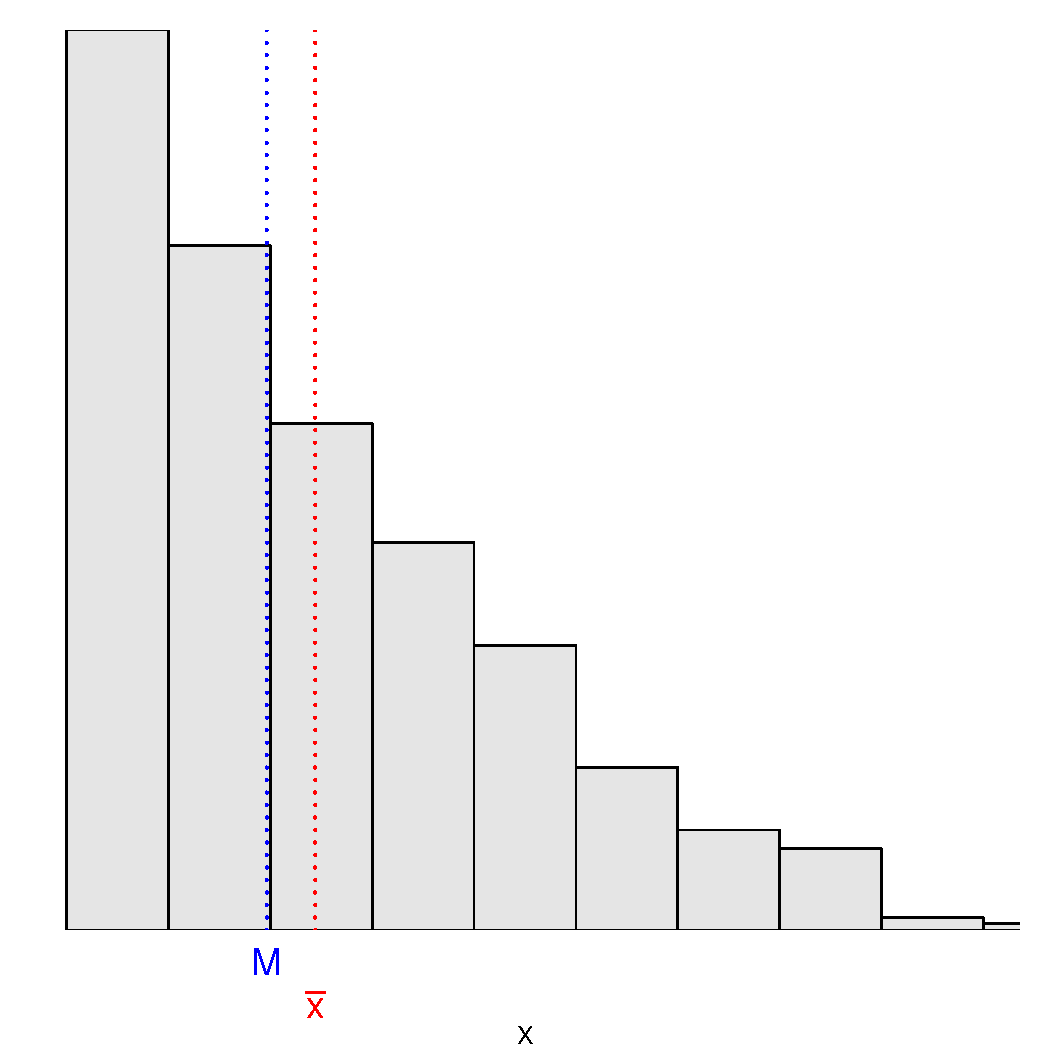
\includegraphics[width=.3\linewidth]{figure/MeanMedianShape-2} \caption[Three differently shaped histograms with vertical lines superimposed at the median (M]{Three differently shaped histograms with vertical lines superimposed at the median (M; blue lines) and the mean ($\bar{x}$; red lines).}\label{fig:MeanMedianShape2}
\end{figure}

\begin{figure}
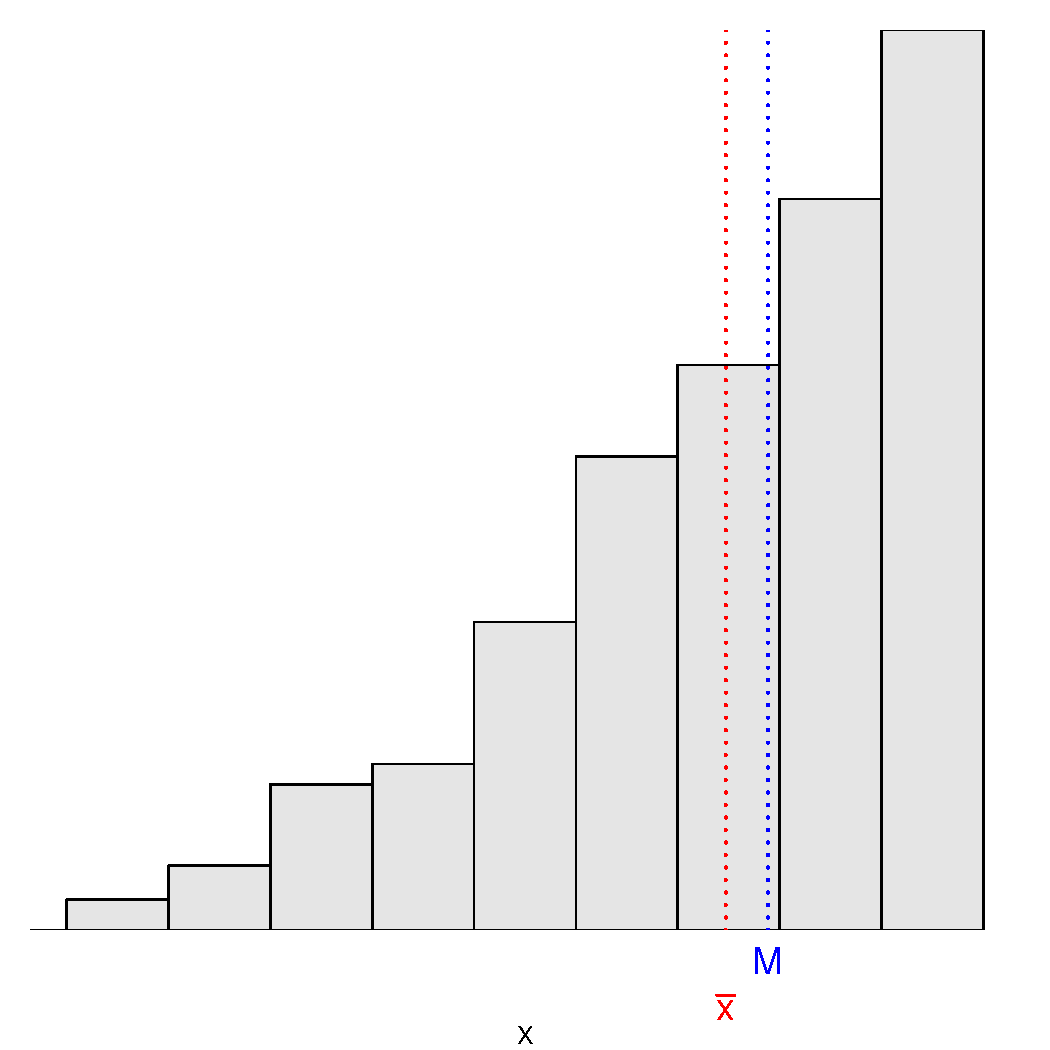
\includegraphics[width=.3\linewidth]{figure/MeanMedianShape-3} \caption[Three differently shaped histograms with vertical lines superimposed at the median (M]{Three differently shaped histograms with vertical lines superimposed at the median (M; blue lines) and the mean ($\bar{x}$; red lines).}\label{fig:MeanMedianShape3}
\end{figure}


\end{knitrout}

\warn{The mean and median are equal for symmetric distributions.}

\vspace{-12pt}
\warn{The mean is pulled towards the long tail of a skewed distribution. Thus, the mean is greater than the median for right-skewed distributions and the mean is less than the median for left-skewed distributions.}

As shown above, the mean and median measure center in different ways. The question now becomes ``which measure of center is better?''  The median is a ``better'' measure of center when outliers are present. In addition, the median gives a better measure of a typical individual when the data are skewed. Thus, in this course, the median is used when outliers are present or the distribution of the data is skewed.\index{Median!When to use}  If the distribution is symmetric, then the purpose of the analysis will dictate which measure of center is ``better.''  However, in this course, use the mean when the data are symmetric or, at least, not strongly skewed.\index{Mean!When to use}

\warn{Describe center with the median if outliers are present or the data are skewed; use the mean if the data are symmetric and no outliers are present.}

\vspace{-12pt}
\begin{exsection}
  \item \label{revex:quEDALSkewMM}Is the mean less than, approximately equal to, or greater than the median for the distribution shown in Exercise \ref{revex:quEDALSkewg}? \ansref{ans:quEDALSkewMM}
  \item \label{revex:quEDAAsymMM}Is the mean less than, approximately equal to, or greater than the median for the distribution shown in Exercise \ref{revex:quEDASymg}? \ansref{ans:quEDAAsymMM}
  \item \label{revex:quEDARSkewMM}Is the mean less than, approximately equal to, or greater than the median for the distribution shown in Exercise \ref{revex:quEDARSkewg}? \ansref{ans:quEDARSkewMM}
  \item \label{revex:quEDARatio} Is the mean divided by the median less than 1, equal to 1, or greater than 1 for a symmetric distribution? \ansref{ans:quEDARatio}
  \item \label{revex:quEDABruleMM} From your calculation of the mean and median in Review Exercise  \ref{revex:quEDABrule} do you expect the histogram to be left-skewed, approximately symmetric, or right-skewed? \ansref{ans:quEDABruleMM}
  \item \label{revex:quEDAWIcMM} From your calculation of the mean and median in Review Exercise \ref{revex:quEDAWIc} do you expect the histogram to be left-skewed, approximately symmetric, or right-skewed? \ansref{ans:quEDAWIcMM}
\end{exsection}



\section{Overall Summaries}
Overall numerical summaries come from considering the relationship between measures of center and dispersion. From the previous section it was seen that the standard deviation and mean are conceptually linked, as are the median and IQR. Indeed, the linked measure of center must be computed first in both dispersion calculations. Thus, if the mean is used to measure center, then the standard deviation must be used to measure dispersion.\index{Standard Deviation!When to use}  Similarly, if the median is used to measure center, then the IQR must be used to measure dispersion.\footnote{Recall that the range will never be used by itself.}\index{IQR!When to use}


\section{Example Interpretations}\index{EDA!Univariate!Quantitative}
While most of the previous sections focused on how to construct various graphs and numerical summaries, the most important aspect of this module is that you can make appropriate interpretations for an EDA from the summary results. For quantitative data, an appropriate EDA consists of identifying the shape, center, dispersion, and outliers for the variable. For categorical data, an appropriate EDA consists of identifying the major characteristics among the categories. Below, I model properly constructed EDAs for the mouse consumption data and two new data sets.

\subsubsection{Mouse Consumption Example}
\begin{quote}
\textit{Construct a proper EDA for the following situation and data -- `The  following measurements \tabrefp{tab:MouseData} are of the consumption of water in one hour by mice in a laboratory setting.'}
\end{quote}
\vspace{-12pt}

\begin{knitrout}
\definecolor{shadecolor}{rgb}{0.969, 0.969, 0.969}\color{fgcolor}\begin{kframe}


{\ttfamily\noindent\bfseries\color{errorcolor}{\#\# Error in Summarize(mc, digits = 2): could not find function "{}Summarize"{}}}\end{kframe}
\end{knitrout}













